%!TEX ROOT=main.tex
\chapter{Hardware}
V této sekci je popsán návrh a dokumentace elektro-mechanické části systému pro měření hemodynamických parametrů krevního řečiště pacienta.

\begin{figure}[H]
    \label{fig:block_cardi}
    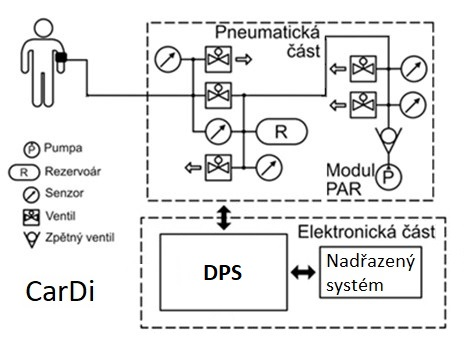
\includegraphics[width=1\textwidth]{pictures/blokove_schema_cele_zarizeni.jpg}
    \caption{Blokové schéma zařízení}
\end{figure}
Součástí pneumatické části je uzavírací ventil, regulační ventily na obou částech uzavíracího ventilu, sensory tlaku, diferenční sensor tlaku, rezervoár a klinicky validovaný modul pro měření krevního tlaku.
K elektronické části patří obvody pro ovládání regulačních a uzavíracího ventilu, komunikace s modulem pro měření tlaku, sběr dat ze sensorů tlaku na obou částech uzavíracího ventilu, komunikace a sběr dat z 24bitového analogově-digitálního převodníku, na který je připojen diferenční sensor tlaku,
uložení a čtení dat do přidané FLASH paměti.
\section{Řídící jednotka}

Řídící jednotka působí jako centrum řízení a sběru dat.
Má na starosti řízení ventilů,
sběr a vyhodnocení dat ze sensorů, komunikaci s modulem pro měření krevního tlaku a komunikaci s nadřazeným systémem. \par

Jako řídící jednotka je vybrán mikroprocesor STM32F407ZG6 (dále jenom MCU) od firmy ST Microelectronics.
Jádro MCU je Arm Cortex-M4 na 32bit architektuře, jehož taktovací frekvence může být až $168 \ MHz$. Jádro Cortex-M4 je vhodné pro zpracování signálu díky zabudovanému výpočetnímu modulu Floating Point Unit (FPU) určené na
počítání s desetinnými čísly a také řadou instrukcí určené specificky na zpracování signálu.
\begin{figure}[H]
    \centering
    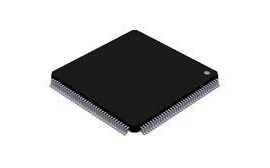
\includegraphics[width=0.5\linewidth]{pictures/stm32f407.jpg}
    \caption{Model STM32F407ZGT6 \cite{cite:STM32F407}}
    \label{fig:stm32}
\end{figure}
MCU je v obalu se 144 piny, ze kterých jsou 114 vstupně/výstupní piny, 1 MB FLASH paměti, 256 kB paměti SRAM, 3x 12 bit AD převodníky s až 24 kanály a maximální vzorkovací frekvencí $2.4 \ MHz$,
2x 12 bit DA převodníky, 14 TIMER, 6x USART, 3x SPI, SysTick Timer, WatchDog a další periferie.
\par
Celkové zapojení MCU je na obrázku (\ref{fig:stm32_conection}).

\begin{figure}[H]
    \centering
    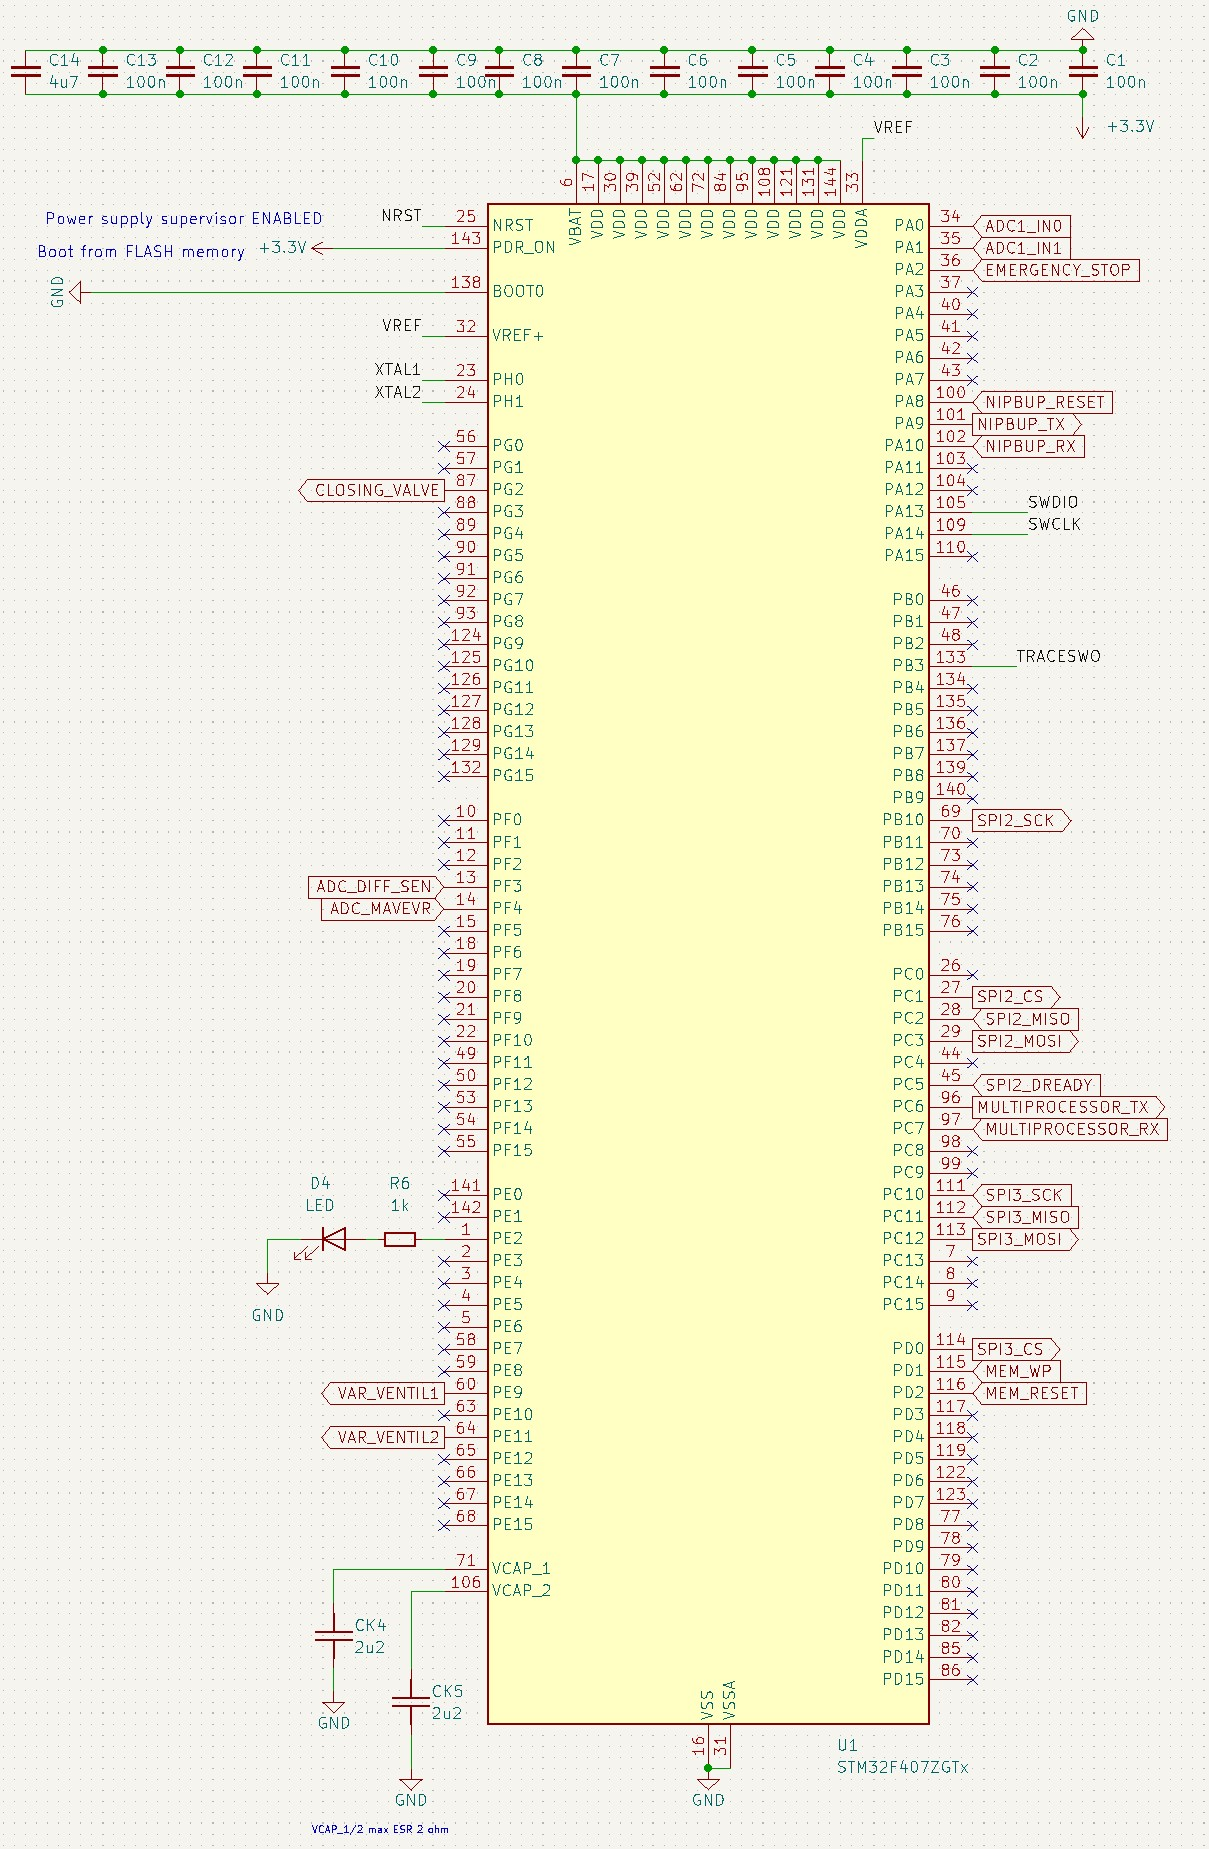
\includegraphics[width=1\linewidth]{pictures/stm_connection.jpg}
    \caption{Schéma zapojení STM32F407ZG}
    \label{fig:stm32_conection}
\end{figure}
\pagebreak
Zapojení MCU je podle doporučeného zapojení z katalogového listu. Jedná se hlavně o umístění a typy blokovacích kondenzátorů, reset signál, boot z interní nebo externí flash paměti a zvolení externích nízko a vysoko kmitočtových hodin. \par

\subsection{Externí hodiny}

MCU obsahuje interní vysokorychlostní RC oscilátor, ale pro maximální přesnost a spolehlivost byl zvolen externí vysokorychlostní oscilátor Abracon ABM3 o frekvenci  $8 \ MHz$. Externí oscilátor slouží jako taktovací hodiny pro
jádro.
Pomocí vnitřní smyčky fázového závěsu (Phase Locked Loop) jádro může být taktováno až na frekvenci $168 \ MHz$.
Snížení frekvence externích taktovacích hodin omezíme vysoko frekvenčního rušení, případného přeslechu na vodičích a celkové zlepšení signálové integrity.
\begin{figure}[H]
    \centering
    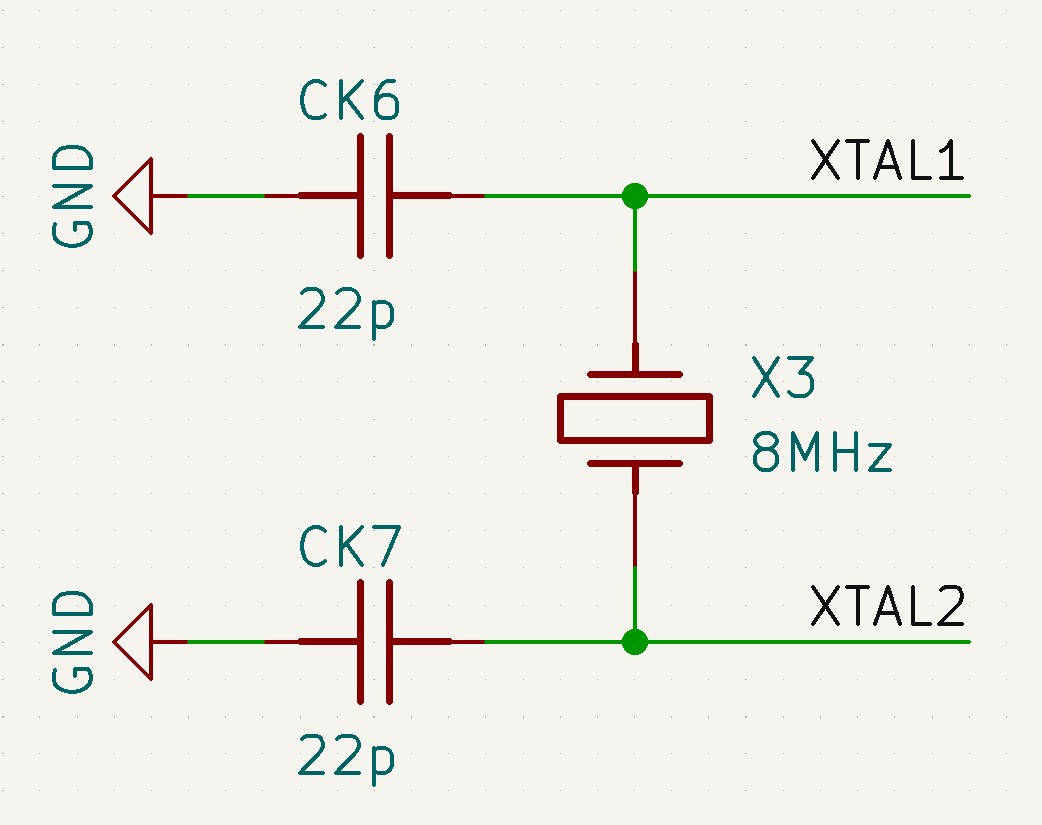
\includegraphics[width=0.8\linewidth]{pictures/stm32_hse.jpg}
    \caption{Schéma zapojení vysokorychlostního externího oscilátoru pro STM32}
    \label{fig:stm32_hse}
\end{figure}


\pagebreak
\subsection{Napěťová reference pro analogové periferie mikroprocesoru} \label{section:vref}
Pro dosáhnutí nejpřesnějšího měření, je třeba, aby analogová část byla co nejméně zarušena. Díky vysokým kmitočtům digitální části MCU může zarušit analogové periférie a proto jsou v MCU digitální a analogové obvody oddělené.
Jako referenční napětí je použito zapojení na obrázku (\ref{fig:stm32_vref}).

\begin{figure}[H]
    \centering
    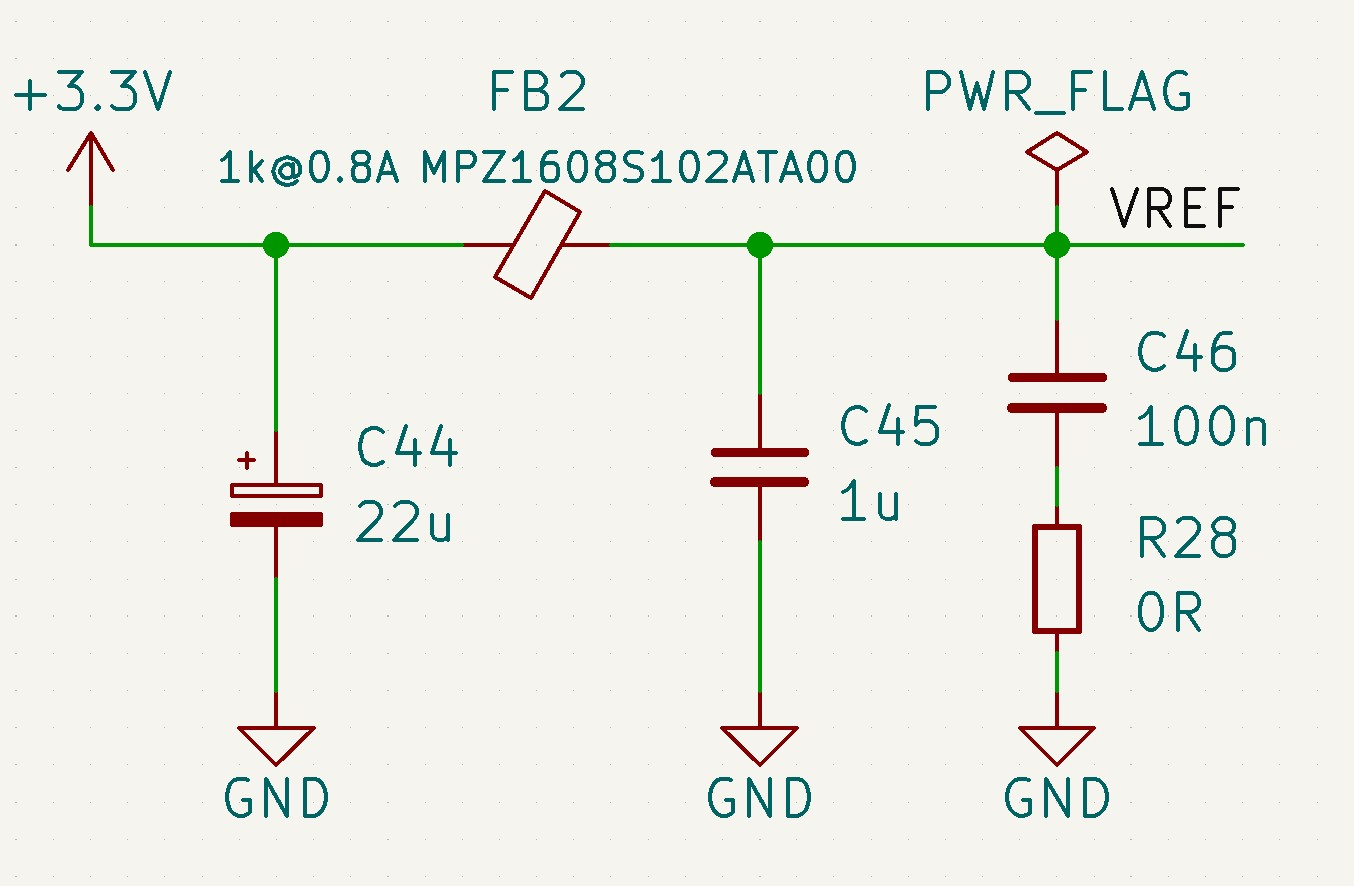
\includegraphics[width=0.9\linewidth]{pictures/stm_analog_reference.jpg}
    \caption{Schéma zapojení referenčního napájení pro analogové periférie MCU}
    \label{fig:stm32_vref}
\end{figure}

\begin{figure}[H]
    \caption{Aproximace frekvenční charakteristiky filtru pro referenční napájení analogové periférie MCU.}
    \label{fig:stm32_vref_response}
    \begin{tikzpicture}
        \begin{axis}[
                width=\linewidth,
                xmode = log,
                ylabel = {(dB)},
                xlabel = {$f$ (Hz) },
                grid=both, % Display a grid
                grid style={dashed,gray!30}, % Set the style  
            ]
            \addplot[width=1pt,color=blue] table {graphs/vref_filtering_cardi.dat};
        \end{axis}
    \end{tikzpicture}
\end{figure}
LC filtr začne potlačovat na frekvenci $f = 138 \ kHz$, ale mezi $\approx 50 \ kHz$ a $ \approx 115 \ kHz$ zesiluje.
Rezonanční frekvence LC filtru je dána vzorcem uvedený níže
\begin{equation}
    f = \frac{1}{2 \pi \sqrt{LC}}
\end{equation}
Výsledná rezonanční frekvence je $f = 89106.66 \ kHz$ o amplitůdě $19 \ dB$.

\subsection{Ochrana proti elektrostatickému výboji}
Elektrostatický výboj (ESD) je náhlý a krátkodobý elektrický proud mezi dvěma objekty s různým elektrickým potenciálem. Představuje hrozbu elektrickým komponentům ve formě trvalého, nevratného poškození. Nejčastější místa probití jsou zejména místa, kterých se často dotýkáme například konektory.
\par
Jako ochrana je použita transient voltage suppression (TVS) dioda D5V0F1U2S9-7 od firmy Diodes Incorporated.

\begin{figure}[H]
    \centering
    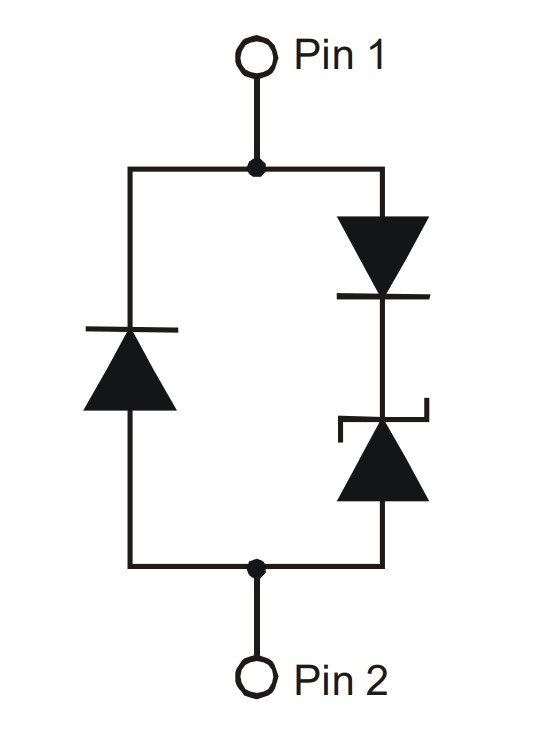
\includegraphics[width=0.4\linewidth]{pictures/esd_diode_schema.jpg}
    \caption{Schéma ochranné ESD diody D5V0F1U2S9-7. Kde Pin 1 je katoda. \cite{cite:ESD}}
    \label{fig:esd_diode}
\end{figure}

Tato dioda je určená pro ochranu proti elektrostatickým výbojům. Je připojena v závěrném směru na všechny konektory. Dioda bude otevřena při zpětném napětí
$U = 5.5 \ V $ a tranzientní napětí omezí na $U_{BR} = 6.0 \ V $.

\section{Modul měření krevního tlaku}

Součástí pneumatické části je modul PAR Medizintechnik NIBP 2020 UP, který umožňuje validované měření krevního tlaku oscilometrickou metodou v průběhu nafukování, také vyfukování, a následné nafouknutí na suprasystolický tlak. Samotné tlakování pneumatického systému je realizováno z elektromechanické vzduchové pumpy integrované v modulu PAR.
Pneumatická část modulu PAR se skládá ze vzduchové pumpy se zpětným ventilem zamezujícím úniku tlaku, vypouštějícího ventilu, tlakového sensoru a také redundantního sensoru tlaku a vypouštěcího ventilu pro případ poruchy. \par
Modul PAR má klinickou validaci pro měření krevního tlaku dle norem EN 80601-2-30, EN 81060-2 a je navržen v souladu norem EN 60601-1 (2. a 3. edice), EN 60601-1-2, EN 60601-1-6.
\begin{figure}[H]
    \centering
    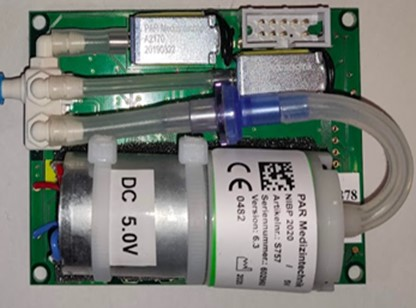
\includegraphics{pictures/par_nibp_up.jpg}
    \caption{Tlakový modul PAR NIBP 2020 UP}
    \label{fig:par_modul}
\end{figure}

Pneumatická část je řízena procesorem, se kterým lze komunikovat pomocí datové sériové linky RS232 či TTL a standardního protokolu CAS s rychlostí 4800 baud. Do modulu jsou posílány přes rozhraní UART příkazy pro nastavení režimu a parametrů, zakončené příkazem pro zahájení měření.
\begin{figure}[H]
    \centering
    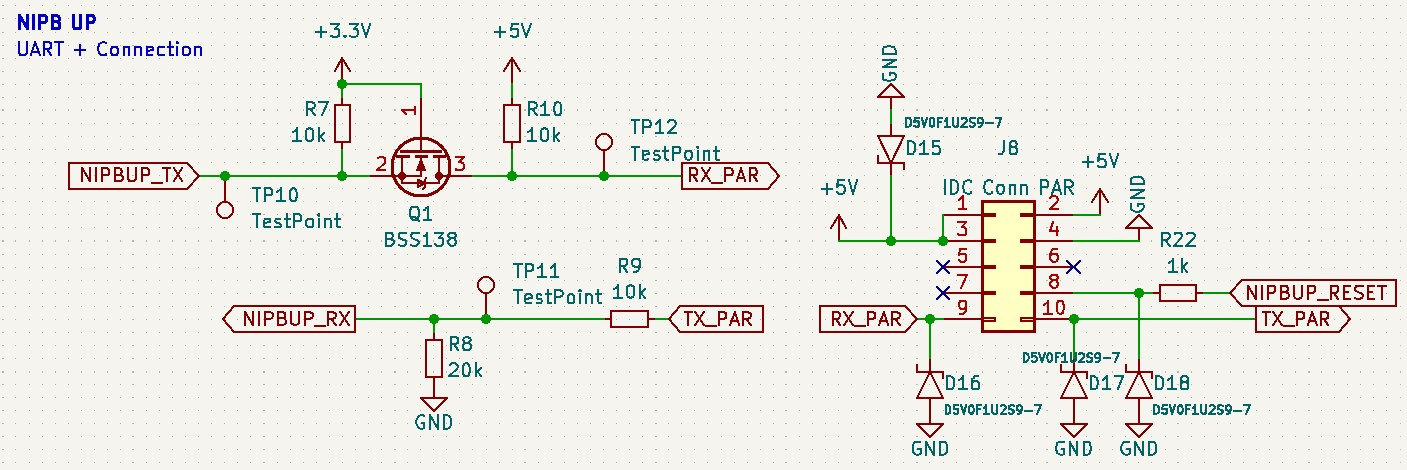
\includegraphics[width=0.9\linewidth]{pictures/nibpup_connection.jpg}
    \caption{Schéma připojení komunikační linky k MCU a napájení pro PAR NIBP 2020 UP }
    \label{fig:par_modul_comm}
\end{figure}
Pneumatickou část lze udržovat na hladinách tlaku v rozmezí (0–300) $mmHg$ po dobu až 180 $s$ a uživateli umožňuje zvolit odstup suprasystolického tlaku od naměřeného systolického tlaku. Po odeslání příkazu pro zahájení měření posílá modul po lince aktuální stav pneumatické části během celého měření a po měření posílá zprávu s naměřenými hodnotami krevního tlaku a srdeční frekvence.
\section{Sensory}
Tato sekce se zaměří na popis a použití sensorů tlaku. Tlakové sensory tvoří nezbytnou část celkového přístroje, rozhodují o přesnosti výsledného měření. \par
Parametry sensorů tlaku vychází z požadavků měření. Pneumatický systém může být pod tlakem až $300 \ mmHg \approx 40 \ kPa$, tento požadavek musí splňovat všechny sensory napojené do pneumatického systému.

\subsection{Sensor tlaku} \label{section:pressure_sen}
Sensor tlaku se používá na snímání tlaku v jednotlivých větvích pneumatického systému. \par

Použité sensory tlaku jsou NPX MP3V5050GC6U.

\begin{figure}[H]
    \centering
    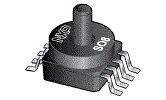
\includegraphics[width=0.5\linewidth]{pictures/nxp_sensor.jpg}
    \caption{sensor tlaku NPX MP3V5050GC6U \cite{cite:NXP}}
    \label{fig:nxp}
\end{figure}

Jedná se o analogový sensor tlaku od firmy NXP ze série peizorezistivních převodníků. Parametry jsou následovné:
\begin{table}[H]
    \label{tab:nxp_properties}
    \caption{Charakteristiky sensoru NPX MP3V5050GC6U. \cite{cite:NXP}}
    \begin{ctucolortab}
        \begin{tabular}{ccccccc}
            \toprule
            Charakteristika                                         & Symbol        & Min & Typ   & Max        & Jednotka         & \\ \midrule
            Rozsah tlaku                                            & $P$           & 0   & -     & 50         & $kPa$            & \\
            Vstupní napětí                                          & $U_{s}$       & 2.7 & 3.0   & 3.3        & $V$              & \\
            Vstupní proud                                           & $I_{s}$       & -   & 7     & 10         & $mA$             & \\
            Napěťový offset($0^{\circ}$ až $ 85^{\circ}  C $)       & $U_{off}$     & -   & 0.188 & -          & $V$              & \\
            $\textnormal{Full Scale Output}^{(\ref{enum:nxp_fso})}$ & $U_{FSO}$     &     & 2.77  &            & $V$              & \\
            Přesnost($0^{\circ}$ až $ 85^{\circ} C$)                & -             & -   & -     & $\pm 2.5 $ & $\%$             & \\
            Citlivost                                               & $\frac{U}{P}$ & -   & 54    & -          & $\frac{mV}{kPa}$ & \\
            \bottomrule
        \end{tabular}
    \end{ctucolortab}

    \begin{enumerate}
        \item \label{enum:nxp_fso} Maximální napětí při největším hodnoceném tlaku.
    \end{enumerate}
\end{table}

Zapojení sensoru je na separátní DPS podle doporučeného zapojení (\ref{fig:nxp_recommended}) z katalogového listu.
\begin{figure}[H]
    \centering
    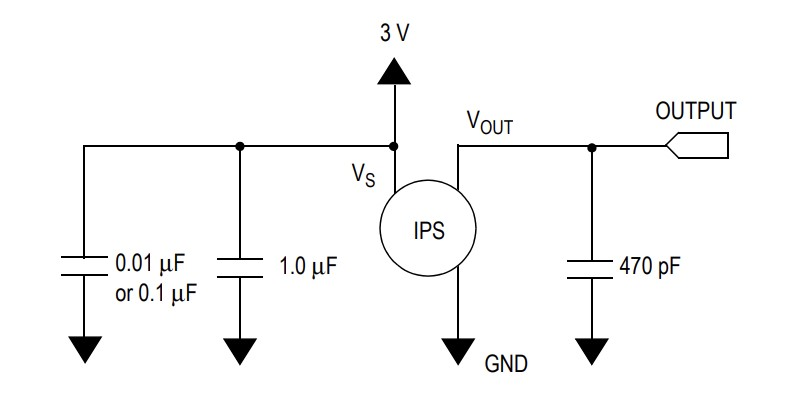
\includegraphics[width=0.9\linewidth]{pictures/nxp_recommended.jpg}
    \caption{Doporučené schéma zapojení sensoru tlaku NPX MP3V5050GC6U. Kde $V_S$ je vstupní napájecí napětí a $V_{out}$ je výstupní napětí.  \cite{cite:NXP}}
    \label{fig:nxp_recommended}
\end{figure}
Analogový výstup ze sensoru je připojen na interní AD převodník MCU.
\subsubsection{Převodní charakteristika}
Převodní charakteristika výstupního napětí $U_{o}$ na tlak $P \ kPa$
\begin{equation}
    P = \frac{U_o \pm ERROR}{0.018 \cdot U_s} - \frac{0.04}{0.018}
    \label{eq:nxp_transfer}
\end{equation}

\begin{figure}[H]
    \centering
    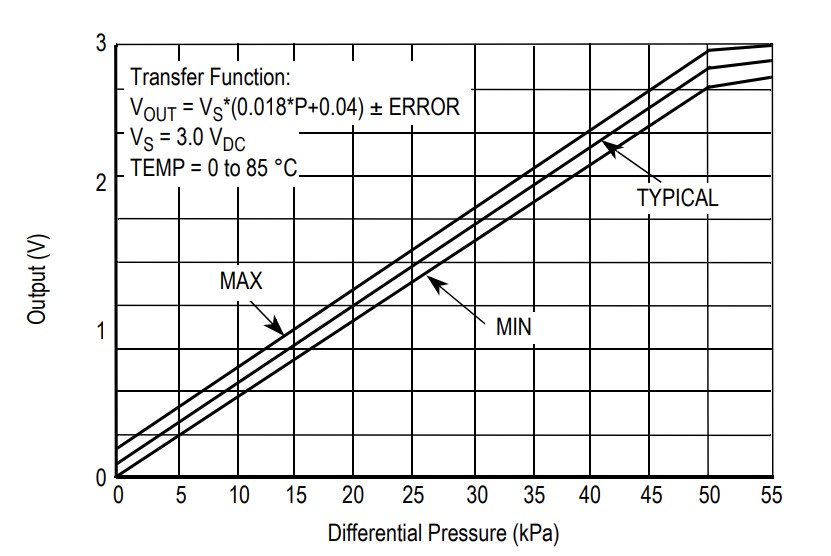
\includegraphics[width=0.9\linewidth]{pictures/nxp_transfer.jpg}
    \caption{Graf převodní rovnice tlak na napětí pro sensor tlaku NPX MP3V5050GC6U. \cite{cite:NXP}}
    \label{fig:nxp_transfer}
\end{figure}

\subsection{Diferenční sensor tlaku} \label{section:diff_pressure_sen}
Diferenční sensor tlaku slouží na snímání malých tlakových pulzací. Porovnává tlak mezí první a druhou (referenční) větví systému. Po natlakování pneumatického systému až na $300 \ mmHg$ uzavírací ventil oddělí systém na dvě větve. Rozdíl tlaků ve větvi může být $300 \ mmHg$ neboli $40 \ kPa$. \par
Diferenční sensor tlaku byl zvolen Amphenol ELVH-L02D-HRRD-C-NAA4. Je to analogový sensor tlaku určený na snímání velmi nízkých tlaků.
\begin{figure}[H]
    \centering
    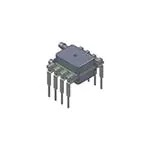
\includegraphics[width=0.4\linewidth]{pictures/amphenol.jpg}
    \caption{Diferenční sensor tlaku Amphenol ELVH-L02D-HRRD-C-NAA4 \cite{cite:Allsensors}}
    \label{fig:amphenol}
\end{figure}


\begin{table}[H]
    \label{tab:amphenol_properies}
    \caption{Charakteristiky diferenčního tlakového sensoru Amphenol ELVH-L02D-HRRD-C-NAA4 \cite{cite:Allsensors}}
    \centering
    \begin{ctucolortab}
        \begin{tabular}{ccccccc}
            \toprule
            Charakteristika                                                         & Symbol    & Min     & Typ               & Max         & Jednotka & \\ \midrule
            Rozsah tlaku                                                            & $P$       & -497.68 & -                 & 497.68      & $Pa$     & \\
            $\textnormal{Proof pressure}^{(\ref{enum:amp_proof_pressure})}$         & $P_{pp}$  & -       & 67                & -           & $kPa$    & \\
            $\textnormal{Průrazný tlak}^{(\ref{enum:amp_burst_pressure}) }$         & $P_{bp}$  & -       & 103               & -           & $kPa$    & \\
            $\textnormal{Common mode pressure}^{(\ref{enum:amp_common_pressure})} $ & $P_{cm}$  & -       & 103               & -           & $kPa$    & \\
            Vstupní napětí                                                          & $U_{s}$   & 3.0     & 3.3               & 5.0         & $V$      & \\
            Vstupní proud                                                           & $I_{s}$   & -       & 2.1               & 2.8         & $mA$     & \\
            Napěťový offset                                                         & $U_{off}$ & -       & 1.65              & -           & $V$      & \\
            $\textnormal{Full Scale Span}^{(\ref{enum:amp_fss})} $                  & $U_{FSS}$ &         & $\pm 40 \% \ U_s$ &             & $V$      & \\
            Přesnost                                                                & -         & -       & -                 & $\pm 0.25 $ & $\%$     & \\
            Citlivost                                                               & -         & -       & 0.2               & -           & $\%$     & \\
            \bottomrule
        \end{tabular}
    \end{ctucolortab}
    \begin{enumerate}
        \item \label{enum:amp_proof_pressure} Maximální tlak, který může být aplikován na jeden z portů sensoru a zachoval původní specifikace.
        \item \label{enum:amp_burst_pressure} Maximální tlak, který může být aplikován na jeden z portů sensoru, bez způsobení úniku tlaku.
        \item \label{enum:amp_common_pressure} Maximální tlak, který může být aplikován na oba porty zároveň, bez způsobení úniku tlaku.
        \item \label{enum:amp_fss} Algebraický rozdíl napětí při nejmenším možném specifikovaném tlaku a při maximálním specifikovaném tlaku.
    \end{enumerate}
\end{table}
\subsection{Převodní charakteristika}
Sensor má převodní funkci $10 \% - 90 \%$ napěťového rozsahu. Nejmenší možný signál vycházející ze sensoru bude o velikosti $10\% U_s$,
to připadá tlaku $P_{min} = -3.736873 \ mmHg$, největší $90\% U_s$ a výsledný tlak $P_{max} = 3.736873 \ mmHg$.
Sensor má lineární převodní funkci pro převod výstupního napětí na tlak v jednotkách $mmHg$ a je uvedena níže
\begin{equation}
    P = 2.831 \times U - 4.671
\end{equation}
\subsection{Vstupní filtr}
Analogový signál ze sensoru je připojen k 24bitovému AD převodníku přes RC článek. Schéma zapojení k AD převodníku je (\ref{fig:amphenol_circuit})

\begin{figure}[H]
    \centering
    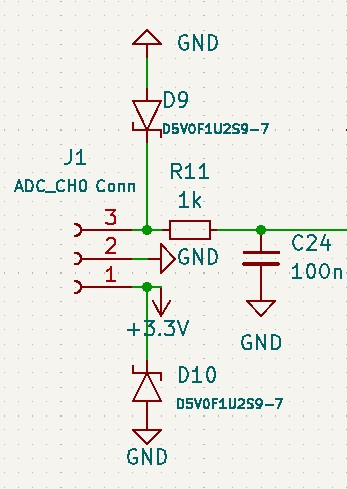
\includegraphics[width=0.7\linewidth]{pictures/diff_sen_circuit.jpg}
    \caption{Schéma zapojení diferenčního sensoru tlaku Amphenol ELVH-L02D-HRRD-C-NAA4 k AD převodníku.}
    \label{fig:amphenol_circuit}
\end{figure}

Při srdečním tepu např. $120 \  \frac{tepů}{min}$ tj. $2 \ Hz$, odpovídá 20. harmonická složka signálu frekvenci  $f = 40 \ Hz$. Pro dodržení Nyquistova vzorkovacího teorému a zachování dynamických vlastností tlakové vlny je zvolena zlomová frekvence RC článku $f_0 = \frac{1}{2 \pi RC} = 1591 \ Hz $.

\begin{figure}[H]
    \centering
    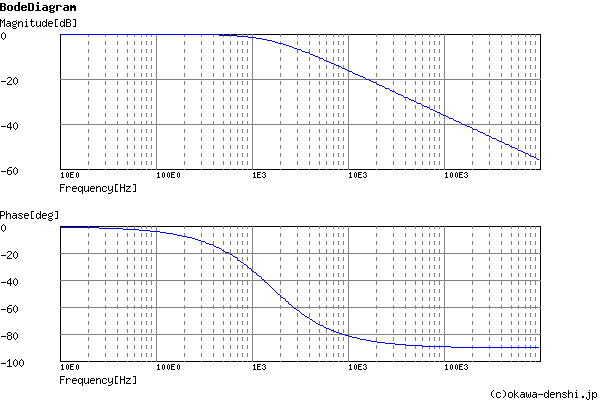
\includegraphics[width=0.9\linewidth]{pictures/rc_1k_100n_1591.png}
    \caption{Bodeho aproximace RC článku pro Amphenol ELVH-L02D-HRRD-C-NAA4. \cite{cite:RCResponse}}
    \label{fig:amphenol_filter}
\end{figure}

\section{Vzduchové ventily}
Ventily jsou důležitou součástí pneumatického systému, starají se o správný průběh měření a také o bezpečí pacienta. \par
V systému rozlišujeme dva druhy vzduchových ventilů, uzavírací a regulační. Uzavírací ventil slouží pro oddělení manžety a pumpy. Vypouštěcí regulační ventily jsou na obou větvích pneumatického systému, slouží pro regulaci tlaku v systému během měření a také jako nouzové vypouštěcí ventily. \par
Všechny použité ventily nesmí v uzavřeném stavu propustit vzduch až do tlaku $300 \ mmHg$.
\pagebreak
\subsection{Uzavírací ventil}
Uzavírací ventil je důležitou součástí systému, pneumatický systém rozdělí na dvě větve, kde jedna je část s manžetou, na které jsou tlakové pulzace a druhá větev je jako referenční. \par

\begin{figure}[H]
    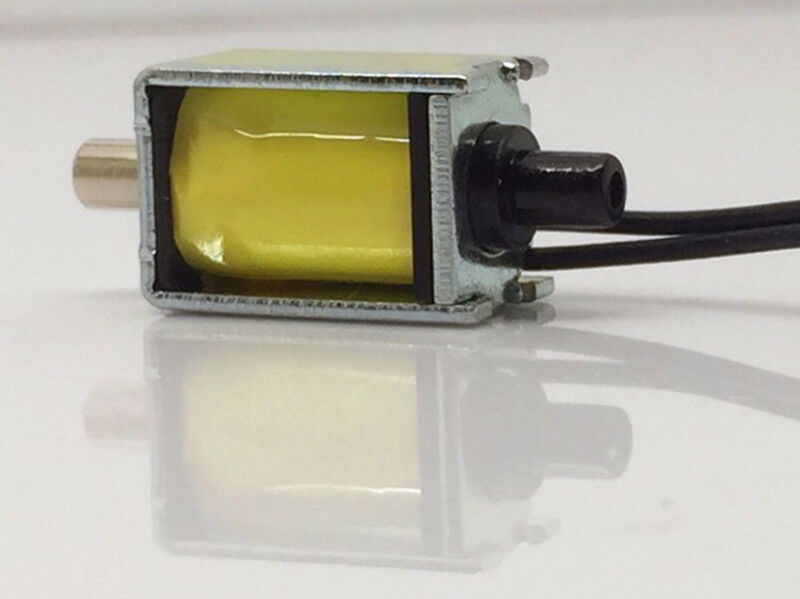
\includegraphics[width=0.9\linewidth]{pictures/closing_valve.jpg}
    \caption{Fotka uzavíracího ventilu CJAV08-2B05A1. \cite{cite:UzaviraciVentil}}
    \label{fig:closing_valve}
\end{figure}

Pro tento účel je použit ventil CONJOIN CJAV08-2B05A1. Je to řízený napětím, normálně zavřený, vzduchový ventil typu solenoid o napájecím napětí $U = 5 \ V$ a vstupním proudu $I = 204 \ mA \pm 10\% $

\begin{figure}[H]
    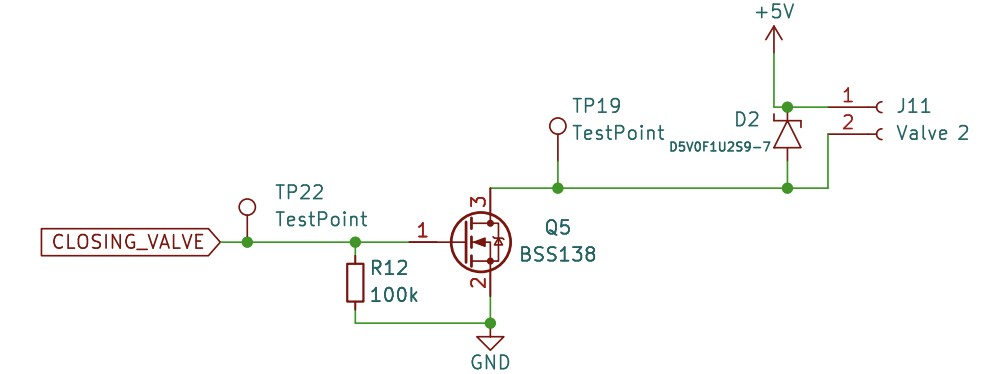
\includegraphics[width=0.9\linewidth]{pictures/closing_valve_driver.jpg}
    \caption{Schéma zapojení uzavíracího ventilu.}
    \label{fig:closing_valve_driver}
\end{figure}

Pro řízení ventilu z výstupního pinu MCU je použitý NMOS tranzistor BSS138. BSS138 má spínací práh napětí $U_{GS} = 3.3 \ V$ což je přímo výstupní napětí z GPIO a maximální proud přes drain je $I_D = 0.22 \ A$.
Rezistor na gate tranzistoru zajisti známé napětí, pokud bude vstup na gate plovoucí, tím se zamezí neznámé chovaní tranzistoru.

\subsection{Regulační ventil}
Regulační ventily slouží k regulaci tlaku v systému při měření a také jako vypouštěcí ventily pro vrácení pneumatického systému na atmosférický tlak. Ventily jsou umístěné na každé větvi pneumatického systému. Během měření je možno si zvolit jak moc vysoký průtok vzduchu je možný, tím můžeme regulovat tlak v obou větvích podle potřeby měření. \par

Použité regulační ventily jsou JQF4-6A/DC6V. Je to normálně otevřený lineární solenoid ventil a maximálním povoleným tlakem $350 \ mmHg$, řízený napětím $U = 6 \ V$ a s proudovým odběrem $I = 107 \ mA$.\par

\begin{figure}[H]
    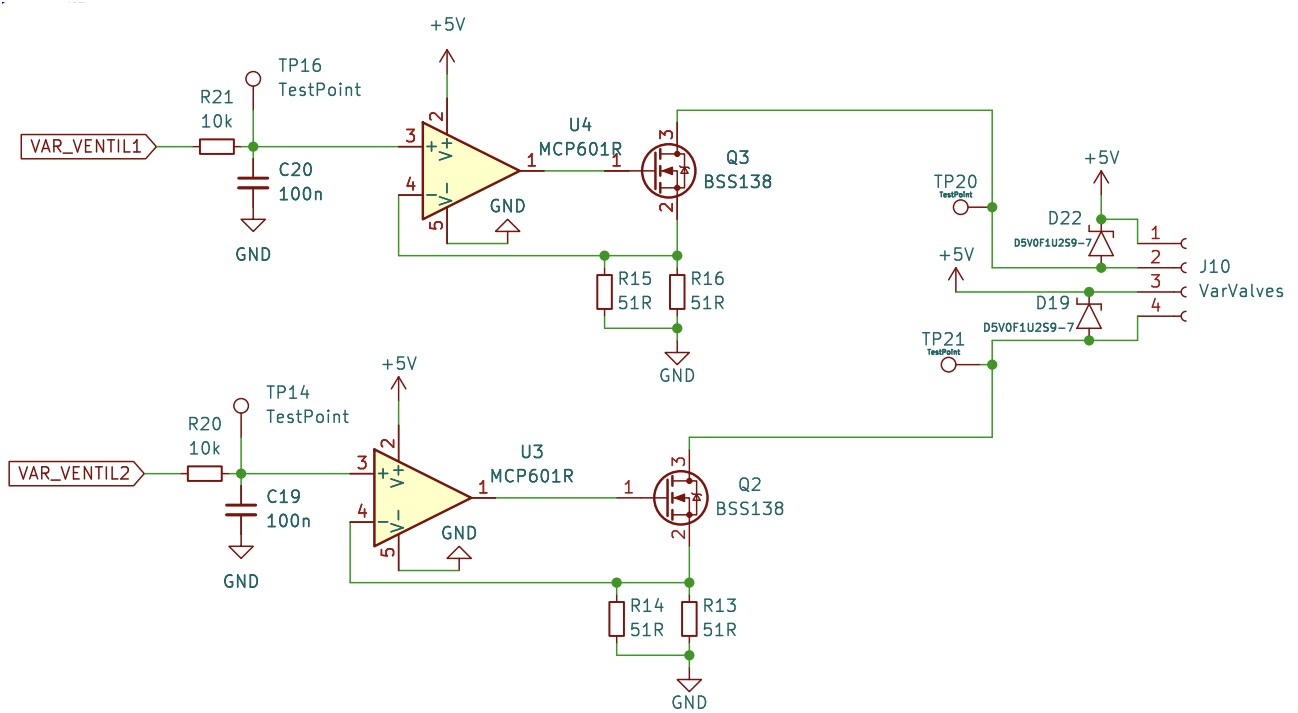
\includegraphics[width=1\linewidth]{pictures/var_valves.jpg}
    \caption{Schéma zapojení regulačních ventilů.}
    \label{fig:variable_valve_driver}
\end{figure}

Napájecí napětí o hodnotě $5 \ V$ bylo zvoleno, po provedení testů, které ukázaly, že zvolené napájecí napětí vyhovuje požadavkům a únik tlaku při plném uzavření nijak neovlivňuje měření a přidáním $6 \ V$ napájení by se zvýšila komplexita návrhu systému.

\subsubsection{Zdroj proudu}
Regulační ventily jsou řízené napěťově řízeným proudovým zdrojem (\ref{fig:variable_valve_driver}).\par
Ventily jsou napojené na drain NMOS tranzistoru, přes který jde konstantní napětí požadované ventilem. Proud se řídí operačním zesilovačem, který má na neinvertujícím vstupu $U_+$ napojené řídící napětí $U_i$. Výstup operačního zesilovače je spojen s gate tranzistoru, source tranzistoru je spojen s invertujícím vstupem $U_-$ operačního zesilovače a také paralelně k zemi jsou zapojené rezistory $R_{||}$, které určují maximální možný proud na regulačních ventilech. Výsledný proud je:
\begin{equation}
    \label{eq:current_source}
    I = \frac{U_i}{R_{||}}
\end{equation}
Paralelní rezistory $R_1 = R_2 = 51 \ \Omega$ mají výslednou hodnotu:
\begin{align*}
    R_{||} = \frac{R_1 R_2}{R_1 + R_2} = \frac{51}{2} = 25.5 \ \Omega
\end{align*}
Maximálním napětí, které umožní MCU z GPIO pinu je $3.3 \ V$ proto maximální možný proud na regulačních ventilech je:
\begin{align*}
    I = \frac{U_i}{R_{||}} = \frac{3.3}{25.5} \doteq  129 \ mA
\end{align*}

Pokud budeme brát v úvahu ideální OZ, tak do invertujícího $U_-$ a neinvertujícího $U_+$ vstupu jde nulový proud, kde $U_+ = U_-$ a výstup z OZ je
\begin{align}
    U_o = A(U_+ - U_-)
\end{align}
kde $A \ [-] $ je zesilovační činitel, který se blíží k nekonečnu.
Použitý NMOS tranzistor je BSS138, má minimální prahové napětí $U_{GS(th)} = 0.5 \ V$, to je napětí, při kterém začne protékat proud na drain.
To znamená, že minimální řídící napětí musí být $U_{i} = 0.5 \ V$.


\subsubsection{Řídící signál}
Jako řídící signál pro řízení proudového zdroje je použit PWM signál, který je převeden na konstatní pomocí filtru typu dolní propust. PWM je generováno z MCU o frekvenci $f_{PWM} = 168 \ kHz$, který je filtrován pomocí RC článku o zlomové frekvenci $f_c = 159 \ Hz$, který slouží pro modulaci řídícího PWM signálu na konstantní napětí.
\par
Pulse Width Modulated (PWM) je periodický čtvercový signál s fixní periodou a měnící se poměrem času v log. 1 a log. 0, také nazývané jako střída (Duty Cycle). Průměrné napětí PWM signálu je
\begin{equation}
    U_{out} = U_{max} \cdot Duty Cycle
\end{equation}
kde $U_{max}$ je maximální amplituda PWM signálu. \par
\begin{figure}[H]
    \centering
    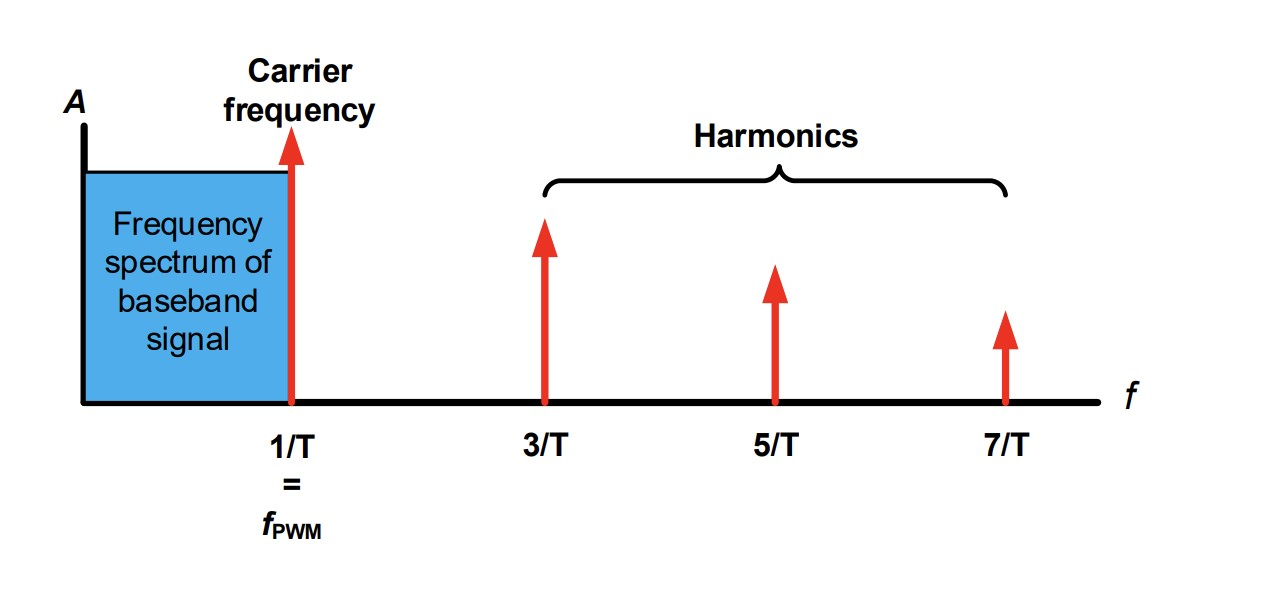
\includegraphics[width=1\linewidth]{pictures/pwm_spectrum_microchip90003250A.jpg}
    \caption{Spektrum PWM signálu převzatého od Microchip TB3250, kde $f_{PWM}$ je frekvence PWM signálu a $T$ je jeho perioda. \cite{cite:MCPPWV}}
    \label{fig:pwm_spectrum}
\end{figure}

Pro převod PWM na konstatní signál je použitý filtr typu dolní propust, jehož zlomová frekvence musí být menší než frekvence PWM signálu.


\begin{figure}[H]
    \centering
    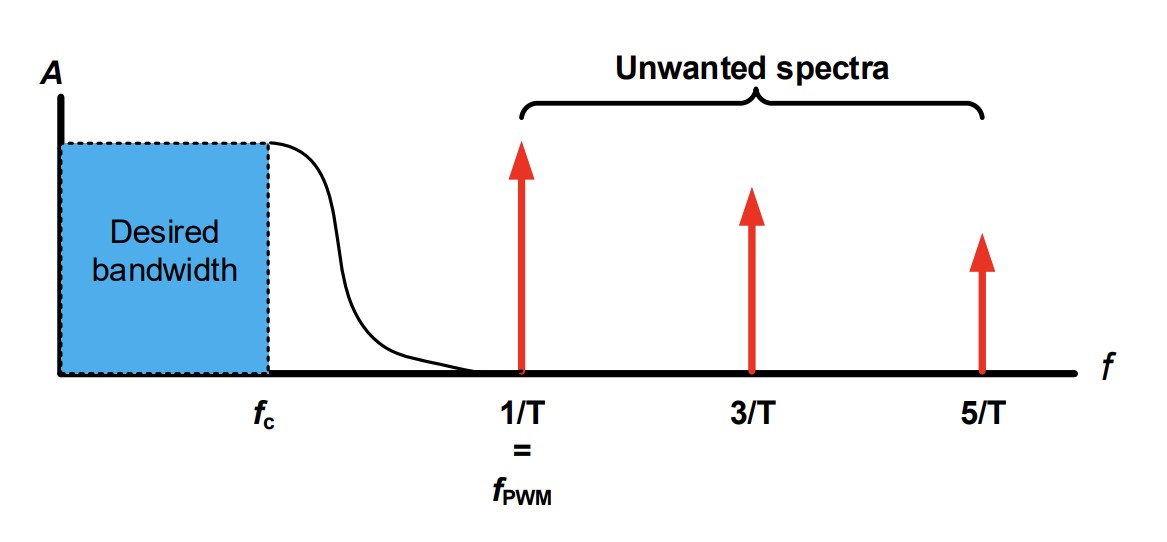
\includegraphics[width=1\linewidth]{pictures/rc_pwm_spectrum_microchip90003250A.jpg}
    \caption{Požadované odstraněné frekvence ve spektru PWM signálu převzatého od Microchip TB3250 kde $f_{PWM}$ je frekvence PWM signálu a $T$ je jeho perioda, $f_{c}$ je zlomová frekvence filtru.\cite{cite:MCPPWV}}
    \label{fig:unwanted_pwm_spectrum}
\end{figure}

Jako filtr typu dolní propust je použit RC článek, který je složen z odporu $R = 10 \ k\Omega$ a kondenzátoru $C = 100 \ nF$, kde výsledná zlomová frekvence filtru je $f_c = 159 \ Hz$.

\begin{figure}[H]
    \centering
    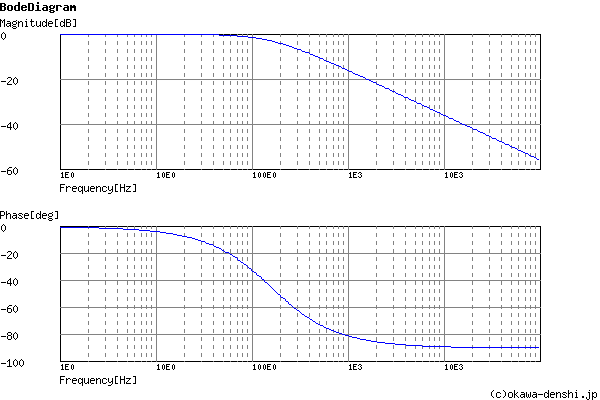
\includegraphics[width=1\linewidth]{pictures/var_rc_filter.png}
    \caption{Frekvenční charakteristika použitého RC filtru pro převod PWV na napětí.\cite{cite:RCResponse}}
    \label{fig:var_rc_filter_char}
\end{figure}

\begin{figure}[H]
    \caption{Simulace RC filtru při vstupním PWM signálu o střídě $50\%$ a frekvencí $f_{PWM} = 168 \ kHz $. Simulace byla provedena v programu LTspice XVII.}
    \label{fig:filtered_pwm}
    \begin{tikzpicture}[spy using overlaysshadow={
                    magnification=3,
                    size=1.5cm,
                    connect spies}
        ]
        \begin{axis}[
                width=0.9\linewidth,
                ytick={0,0.2,...,1.7},
                % title = {Picture 1},  % whatever name you want
                ylabel = {$U_{out}$ (V)},
                xlabel = {Čas (s)},
                grid=major, % Display a grid
                grid style={dashed,gray!30}, % Set the style  
            ]
            \addplot[blue] table {graphs/pwm_to_analog.dat};
            % \begin{scope}
            % \spy [red] on (6,8.5cm) in node at (6.5cm,7.25cm);
            % \spy [blue,size=1cm] on (3cm,1cm) in node  at (0,-1.25cm);
            % \end{scope}
        \end{axis}

    \end{tikzpicture}
\end{figure}

Toto rušení způsobí periodickou změnu amplitudy výstupního signálu a regulační ventil se podle této amplitudy bude periodicky otevírat a zavírat. Při zvolené frekvenci PWM $f_{PWM} = 168000 \ Hz $ je změna napětí $\approx 2 \ mV$, to způsobí změnu proudu $I = \frac{0.002}{25.5} = \pm 78.4 \ \mu A $. \par
Volba velikosti prvků RC článku ovlivní schopnost reakce na změnu vstupního napětí.
Aby napětí na kondenzátoru dosáhlo $\approx 63 \ \% $ vstupního napětí $U_{in}$ bude trvat $\tau = RC = 10 \times 10^{3} \cdot 100 \times 10^{-9}= 1 \ ms$.

\par
Díky rovnici
\begin{equation} \label{eq:pwm_accuracy}
    2^N = \frac{f_{TIMCLK}}{f_{PWM}}
\end{equation}
můžeme získat přesnost střídy PWM signálu. $f_{TIMCLK} = 168 \ MHz$ je obnovovací frekvence periferie TIMER, který generuje PWM signál. Pokud rovnici (\ref{eq:pwm_accuracy}) vyřešme pro $N$ získáme rovnici pro počet bitů a přesnosti střídy PWM signálu.
\begin{equation}
    N = \frac{\log_{2} (\frac{f_{TIMCLK}}{f_{PWM}})}{\log_{2}(2)} = \frac{ARR}{\log_{2}(2)}
\end{equation}
$ARR$ je Auto-Reload-Register MCU pro daný TIMER. Podle nastavené hodnoty v $ARR$ je možné nastavit frekvenci PWM signálu. Pro tento případ $N \doteq 9.96 $ bit.

\section{Digitalizace analogových signálů}
Tato sekce popisuje typy použitých analogově-digitálních převodníků, které jsou použity pro snímání analogových výstupů ze sensorů tlaku. Jsou použity dva typy AD převodníků, první je 12bitový AD převodník součástí MCU STM32F407ZG6 pro snímání napětí tlakových sensorů na větvích pneumatického systému popsaných v sekci (\ref{section:pressure_sen}).
Další je 24bitový sigma-delta AD převodník Microchip MCP3561 pro snímání napětí z diferenčního tlakového sensoru popsaný v sekci (\ref{section:diff_pressure_sen}).

\subsection{Snímání signálů z tlakových sensorů větví pneumatíckého systému}
Je použit AD převodník, který je součástí MCU. Jedná se o 12bitový AD převodník s postupnou aproximací a maximální vzorkovací frekvencí $f_{sample} = 2.4 \ MSPS$. \par
Díky měření pouze absolutní hodnoty tlaku ze sensorů, vzorkovací frekvence nemusí být vysoká. Vzorkovací frekvence je:
\begin{equation}
    f_{sample}=\frac{f_{ADCCKL}}{\textnormal{vzorkovací počet cyklů} + 15 \ \textnormal{cyklů} } = \frac{20.5 \ MHz}{480 + 15} \approx 41.5 \; kHz
\end{equation}
Vzorkovací frekvence závisí na vstupní frekvenci AD převodníku $f_{ADCCKL} = 20.5 \ MHz$, minimální počet $f_{ADCCKL} $ cyklů a vzorkovacím počtem cyklů, které jsou předem dané výrobcem. Minimální počet vzorkovacích cyklů je $3$ a maximální je $480$.
\par
Přesnost AD převodníku je $1 \ LSB = \frac{U_{ref}}{2^N} = \frac{3.3}{2^{12}} = 805 \ \mu V$ závisí na referenčním napětí diskutovaném v sekci (\ref{section:vref}).

\begin{equation} \label{eq:max_adc_R}
    R_{AIN} = \frac{k - 0.5}{f_{ADCCLK} \cdot C_{ADC} \cdot ln(2^{N+2})} - R_{ADC}
\end{equation}
Rovnice (\ref{eq:max_adc_R}) slouží pro určení maximální vstupní impedance pro zaručení chyby převodu pod $\frac{1}{4} \ LSB$. $N = 12$ je rozlišení AD převodníku, $k = 480$ je vzorkovací čas, $R_{ADC} = 6 \ k\Omega$ je vnitřní impedance vstupního kanálu AD převodníku a
$C_{ADC} = 4 \ pF$ je interní kapacita obvodu Sample and Hold. Výsledná maximální vstupní impedance je $R_{AIN} = 1.75 \ M\Omega$, ale podle katalogového listu je maximální externí impedance AD převodníku $R_{AIN} = 50 \ k\Omega$.
\par
K dalším chybám AD převodníku patří pametry níže uvedené v tabulce

\begin{table}[H]
    \label{tab:stm_adc_error}
    \caption{Charakteristika vestavěného AD převodníku v STM32F407ZG6}
    \hspace*{-1.3cm}
    \begin{ctucolortab}
        \begin{tabular}{ccccccc}
            \toprule
            Charakteristika               & Symbol & Testovací podmínky       & Typ       & $\textnormal{Max}$ & Jednotka & \\ \midrule
            Celková neupravená chyba      & $ET$   &                          & $\pm$ 2   & $\pm$ 5            &          & \\
            Napěťová nesymetrie           & $EO$   & $f_{ADC} = 30 \ MHz$     & $\pm$ 1.5 & $\pm$ 2.5          &          & \\
            Napěťový zisk                 & $EG$   & $R_{AIN} < 10 \ k\Omega$ & $\pm$ 1.5 & $\pm$ 3            & LSB      & \\
            Difereciální  chyba linearity & $ED$   &                          & $\pm$ 1   & $\pm$ 2            &          & \\
            Integrální chyba linearity    & $EL$   &                          & $\pm$ 1.5 & $\pm$ 3            &          & \\
            \bottomrule
        \end{tabular}
    \end{ctucolortab}
\end{table}

\subsection{Snímání signálů z diferenčního tlakového sensoru pneumatíckého systému} \label{section:mcp3561_hw}
Diferenční sensor tlaku snímá dynamické jevy tlakových pulzací. Při srdečním tepu např. $120 \ \frac{tepů}{min}$ tj. $2 \ Hz$, odpovídá 20. harmonická složka signálu frekvenci  $f = 40 \ Hz$. Aby byl tlakový analogový signál správně převeden do digitálního signálu, musí být dodržen Nyquistův teorém.
\begin{equation} \label{eq:nyquist}
    f_s \geq 2f
\end{equation}
Rovnice (\ref{eq:nyquist}) říká, že vzorkovací frekvence musí být alespoň dvojnásobek snímaného signálu.
\par
Pro zachycení pulzní tlakové vlny je také zapotřebí dostatečné rozlišení v časové oblasti. Pokud vzorkovací frekvence signálu je $f_s = 5000 \ Hz$, chyba v měření může být $t_e = \pm 200 \ \mu s$. Podle vzorce (\ref{eq:pwv}) můžeme vypočítat chybu měření PWM v závislosti na časovém kroku.
Například ať $l = 0.5 \ m$, $t_2 = 200 \ ms$ a $t_1 = 0 \ ms$, výsledné $PWV$ bude $PWV = 5 \ \frac{m}{s}$. Pokud započítáme chybu $t_e$ do výpočtu rychlost šíření pulzní vlny bude
\begin{equation*}
    PWV = \frac{2l}{t_2 - t_1 + t_e} = \frac{1}{0.2 - 0.0002} = 5.005 \ \frac{m}{s}
\end{equation*}
\begin{equation*}
    PWV = \frac{2l}{t_2 - t_1 + t_e} = \frac{1}{0.2 + 0.0002} = 4,995 \ \frac{m}{s}
\end{equation*}
Výsledek se může lišit o $\pm 0.1 \ \%$.
\par
Byl vybrán 24bitový sigma-delta AD převodník MCP3561 od firmy Microchip s maximální vzorkovací frekvencí $153.6 \ kHz$. Je to AD převodník s velmi nízkým šumem, s jedním diferenčním vstupem nebo dvěma jednotlivými vstupy analogových signálu,
obsahuje interní oscilátor, teplotní sensor, obvody pro detekci zkratu či odpojeného sensoru, programovatelné zesílení od $0.33 \times$ až $64 \times$ a další.
\par
MCP3561 komunikuje s MCU pomocí komunikačního rozhraní Serial Peripheral Interface (SPI) až s maximální rychlostí $20 \ MHz$. Komunikace probíhá po 8 bitových slovech, kde odpovědi z AD převodníku můžou mít délku 8, 24 a nebo podle konfigurace i 32 bit.
\begin{figure}[H]
    \centering
    \caption{Zapojení AD převodníku MCP3561}
    \label{fig:mcp3561_connection}
    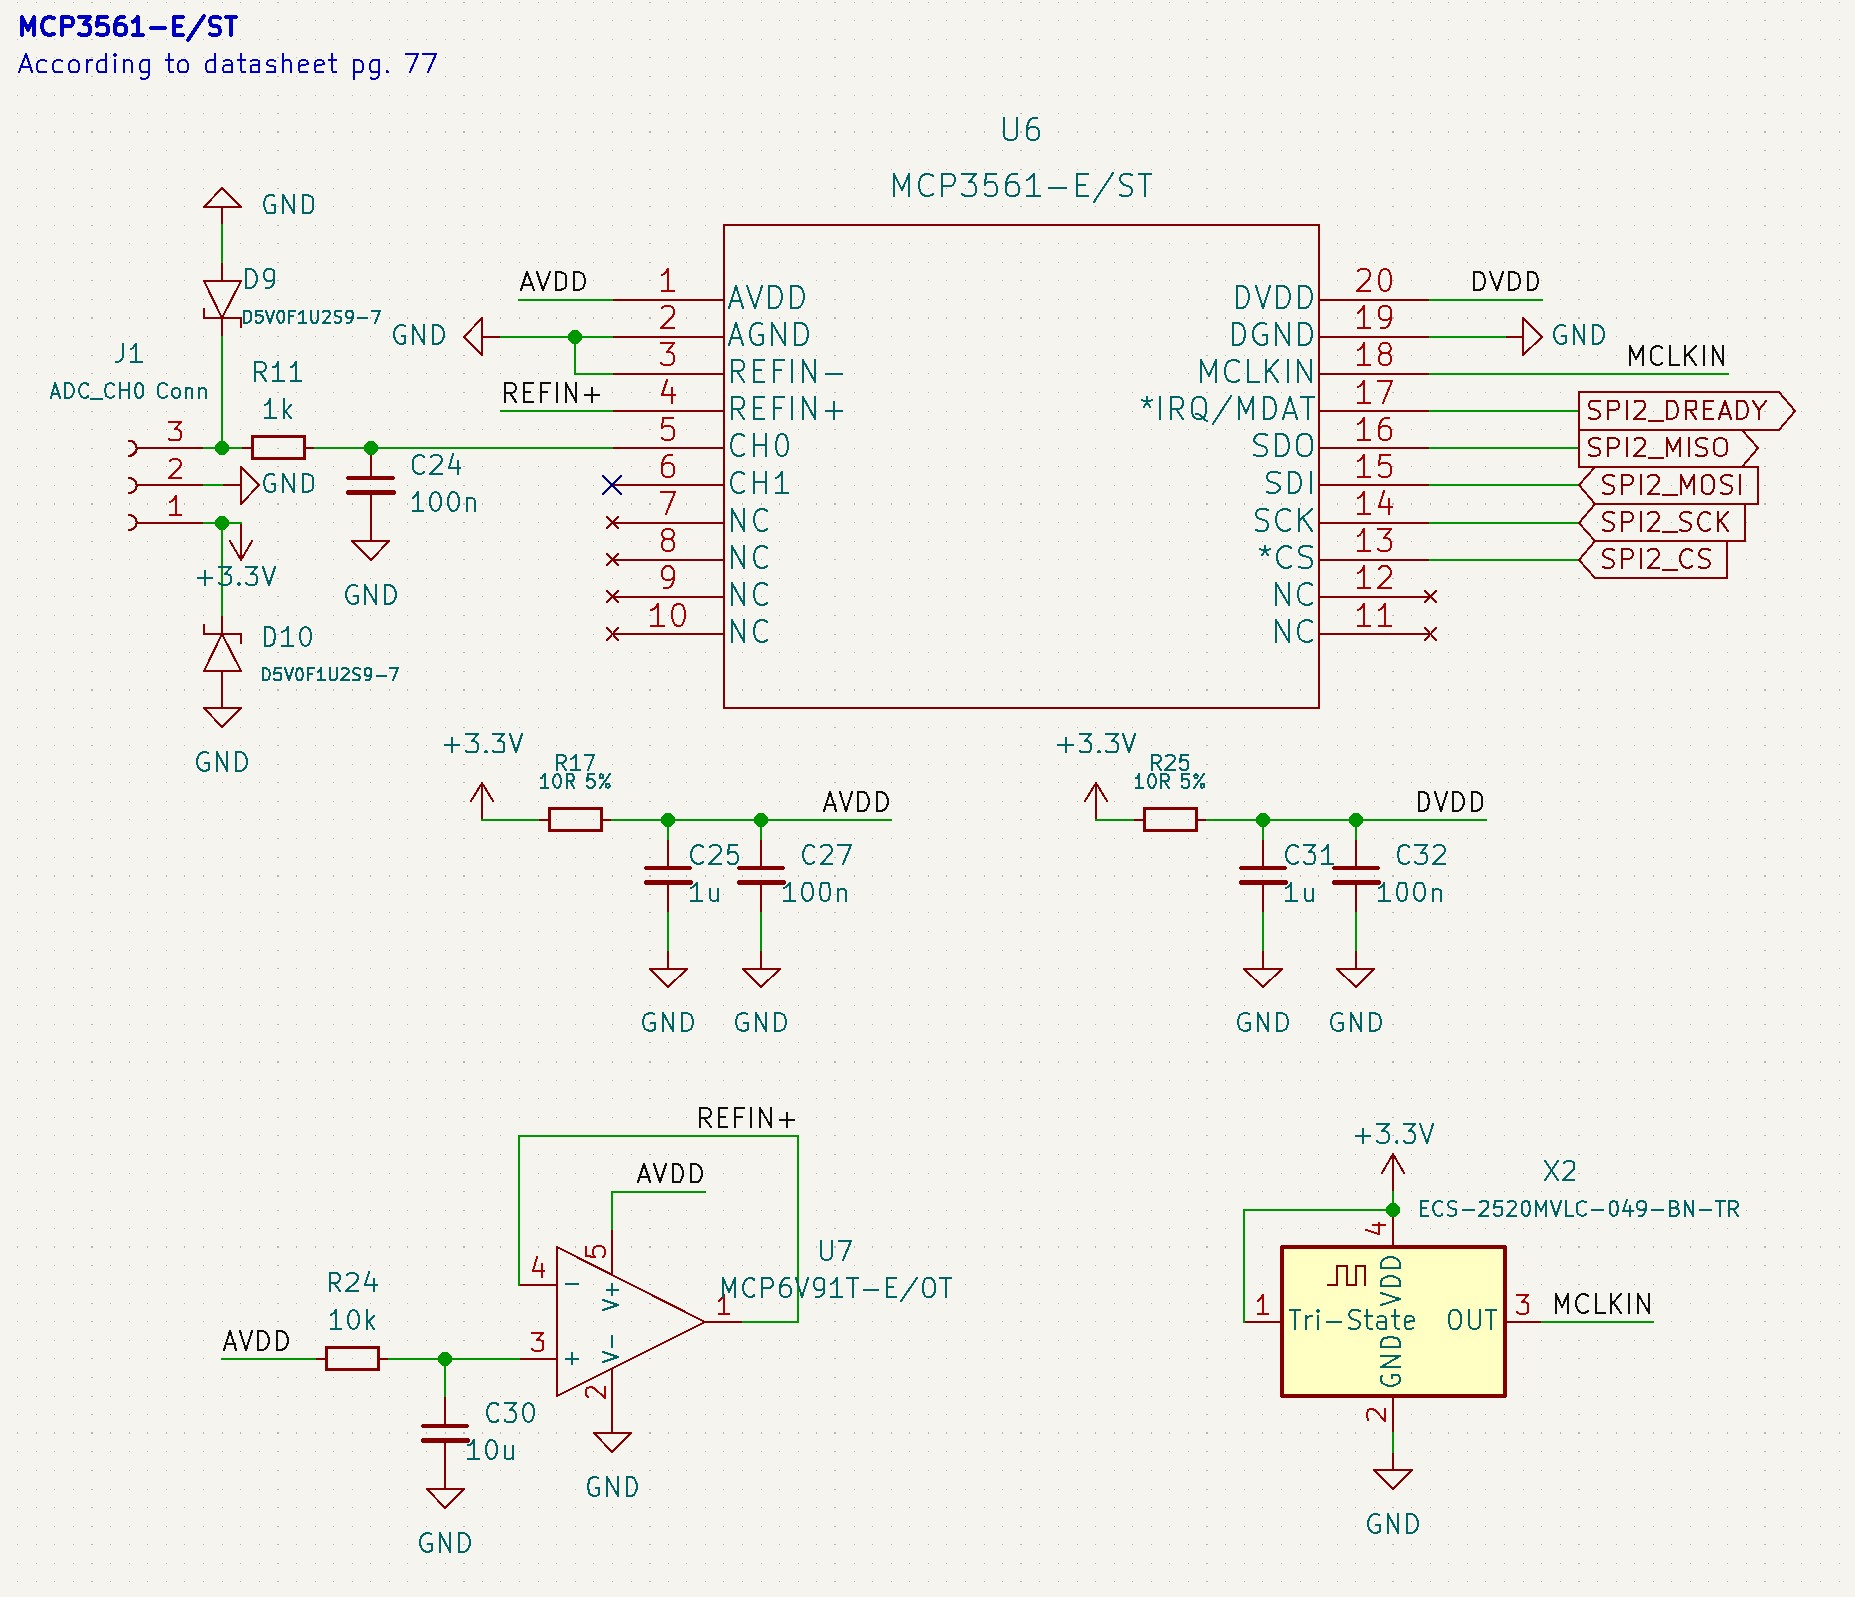
\includegraphics[width=1\linewidth]{pictures/mcp3561_connection.jpg}
\end{figure}
\subsubsection{Napájení a napěťové reference}
Zapojení obsahuje oddělené filtrování napájení analogové a digitální reference AD převodníku. Použitý filtr je RC článek typu dolní propusti s parametry rezistoru $R = 10 \ \Omega$ a kondenzátoru $C = 1100 \ nF$, kde zlomová frekvence RC článku je $f_c \doteq 14.5 \ kHz$.
\par
Referenční analogové napájení AD převodníku obsahuje operační zesilovač v zapojení napěťového sledovače, protože není impedančně oddělená. Operační zesilovač je MCP6V91T od firmy Microchip s nízkou teplotně závislou napěťovou nesymetrii $U_{OS \ Drift} = \pm 17  \ \frac{nV}{^\circ C}$
a také nízkou napěťovou nesymetrii $U_{OS} = 9 \ \mu V$, nízký šum a je optimalizovaný pro použití v prostředí s vysokým elektromagnetickým rušením.

\subsubsection{Externí oscilátor}
Místo interního oscilátoru AD převodníku je použit externí oscilátor ECS-2520MVLC od firmy ECS Inc. s frekvencí $f_{CLK} = 4.9152 \ MHz$. Externí oscilátor zaručí stabilní funkčnost AD převodníku, protože přesnost interního oscilátoru není výrobcem zaručena, s frekvenčními rozdíly až $\pm 30  \ \%$.
Podporované frekvence externího oscilátoru jsou v rozmezí $ 1 \ MHz \leq  f_{CLK} \leq 20 \ MHz $. Frekvence $f_{CLK} = 4.9152 \ MHz$ byla zvolena díky naměřeným parametrů AD převodníku v katalogovém listu při této frekvenci.
\par
Maximální možná přenosová rychlost pro tuto frekvenci oscilátoru je $f_s = 38400 \ Hz$.

\subsubsection{Přesnost a rušení}
Nejmenší možné snímané napětí ideálního $N = 24$ bit AD převodníku, při referenčním napětí $U_{ref} = 3.3 \ V $ je $ 1 \ LSB = \frac{U_{ref}}{2^{N-1}} \doteq 393.39 \ nV$. N-1 je protože rozsah snímaného napětí je $\pm U_{ref}$ a největší bit je rezervován pro znaménko.
Efektivní počet bitů (ENOB) závisí na interní konfiguraci registrů MCP3561 a od toho se také odvíjí, jaká přenosová rychlost bude mít nejlepší počet efektivních bitů. Přenosová rychlost udává počet vzorků odeslané po přenosové lince nadřazenému systému, signalizovaném výstupním digitálním pinem AD převodníku $\overline{IRQ}$.
Rovnice po výpočet přenosové rychlosti:
\begin{equation}
    f_s = DRCLK = \frac{DMCLK}{OSR} =\frac{f_{CLK}}{4 \times OSR \times PRESCALE}
\end{equation}
Rovnice je převzána z katalogového listu AD převodníku, kde $f_{CLK} = 4.9152 \ MHz$ je frekvence AD převodníku, DMCLK je vzorkovací frekvence AD převodníku, PRESCALE je hodnota pro decimaci taktovací frekvence AD převodníku s hodnotami $PRESCALE = \{1, 2, 4, 8\}$, OSR (Oversampling Ratio) je poměr vzorkovací frekvence ku přenosové rychlosti.
Počet efektivních bitů a rušení na OSR, čím vyšší OSR, tím větší bude počet použitelných bitů a menší rušení. Pro dosáhnutí přenosové rychlosti $f_s = 5000 \ Hz$ byly vybrány hodnoty $PRESCALE = 1$, $OSR = 256$ a zesílení $GAIN = 1$,
vzorkovací frekvence AD převodníku je $DMCLK = \frac{f_{CLK}}{4 \times PRESCALE} = 1 \ 228 \ 800 \ Hz$ a výsledná přenosová rychlost je $f_s = DRCLK = 4800 \ Hz$ s $ENOB = 19.5 \ bit$ a RMS rušení $U_{noise \ RMS} = 8.94 \ \mu V$.
Výsledná přesnost AD převodníku se sníží na $ 1 \ LSB = \frac{U_{ref}}{2^{ENOB}} \doteq  4.4 \ \mu V$.
\par
Dalším parametry AD převodníku MCP3561 jsou níže uvedené tabluce
\begin{table}[H]
    \label{tab:mcp_adc_error}
    \caption{Charakteristika AD převodníku MCP3561. }
    % \centering
    \begin{itemize}
        \item $f_{CLK} = 4.9152 \ MHz$, $DU_{DD} = AU_{DD} = U_{REF} = 3.3 \ V$, $T = 25 ^\circ C$
    \end{itemize}
    \hspace*{-2cm}
    \begin{ctucolortab}
        \begin{tabular}{ccccccc}
            \toprule
            Charakteristika                           & Symbol                                   & Min                 & Typ               & $\textnormal{Max}$ & Jednotka                                          & \\ \midrule
            Impedance analogového vstupu              & $Z_{in}^{(\ref{enum:mcp_gain_one})}$     & -                   & 260               & -                  & $k \Omega$                                        & \\
            Rozlišení zavislé na OSR                  & $Rozlišení^{(\ref{enum:mcp_accuracy})}$  & 24                  & -                 & -                  & bit                                               & \\
            Napěťová nesymetrie                       & $U_{OS}$                                 & $\frac{-900}{GAIN}$ & -                 & $\frac{900}{GAIN}$ & $\mu V$                                           & \\
            Napěťová nesymetrie závislá na teplotě    & $U_{OS \ DRIFT}$                         & -                   & $\frac{70}{GAIN}$ & $\frac{300}{GAIN}$ & $\frac{nV}{^\circ C}$                             & \\
            Chyba zesílení                            & $G_E$                                    & -3                  & -                 & +3                 & \%                                                & \\
            Chyba zesílení závislé na teplotě         & $G_{E \ DRIFT}^{(\ref{enum:mcp_drift})}$ & -                   & 0.5               & 2                  & $\frac{ppm}{^\circ C}$                            & \\
            Integrální nelinearita                    & $INL^{(\ref{enum:mcp_gain_one})}$        & -7                  & -                 & +7                 & ppm $\textnormal{FSR}^{(\ref{enum:mcp_adc_fsr})}$ & \\
            Stejnosměrné potlačení souhlasného rušení & $DC \ CMRR$                              & -                   & -126              & -                  & dB                                                & \\
            Střídavé potlačení souhlasného rušení     & $AC \ CMRR$                              & -                   & 122               & -                  & dB                                                & \\
            Poměr signálu k šumu a zkreslení          & $SINAD$                                  & 105.8               & 106.7             & -                  & dB                                                & \\
            Poměr signálu k šumu                      & $SNR$                                    & 106.7               & 107.2             & -                  & dB                                                & \\
            Celkové harmonické zkreslení              & $THD$                                    & -                   & -116              & -111               & dB                                                & \\
            Dynamický rozsah bez parazitních složek   & $SFDR$                                   & 110                 & 120               & -                  & dB                                                & \\
            Přeslech vstupních kanálů                 & $CTALK$                                  & -                   & -130              & -                  & dB                                                & \\
            \bottomrule
        \end{tabular}
    \end{ctucolortab}
    \begin{enumerate}
        \item GAIN = 1 \label{enum:mcp_gain_one}
        \item OSR $\geq$ 256 \label{enum:mcp_accuracy}
        \item GAIN = 1,2,4 \label{enum:mcp_drift}
        \item Full-Scale-Range(FSR) = $2 \times U_{REF}/GAIN$ \label{enum:mcp_adc_fsr}
    \end{enumerate}
\end{table}


\section{Datové úložiště}
Přidané datové úložiště slouží jako úložiště dat z AD převodníku MCP3561. MCU příjmá data o velikosti $N = 24 \ bit$ při přenosové rychlosti $f_s \approx 5000 \ Hz$ po dobu $T = 30 \ s$, minimální velikost úložiště je
\begin{equation*}
    M = N \times f_s \times T = 3 \ 600 \ 000 \ bit
\end{equation*}
Neboli $\frac{M}{8} = 450 \ kB$.
\par
Interní úložiště MCU STM32F407ZG6 typu FLASH je 1 MB, ale slouží pro umístění vektoru přerušení, bootloaderu a programu.
\par
Jako přidané datové úložiště je vybráno NOR FLASH paměť MX25R3235FM2IH0 od firmy Macronix o velikosti 32 Mb. NOR FLASH je typ energeticky nezávislou paměť, po odpojení napájení stále drží zapsaný obsah. Komunikace probíhá přes komunikační protokol SPI.
\begin{figure}[H]
    \label{fig:flash_memory}
    \caption{Schéma zapojení paměti flash Macronix MX25R3235FM2IH0}
    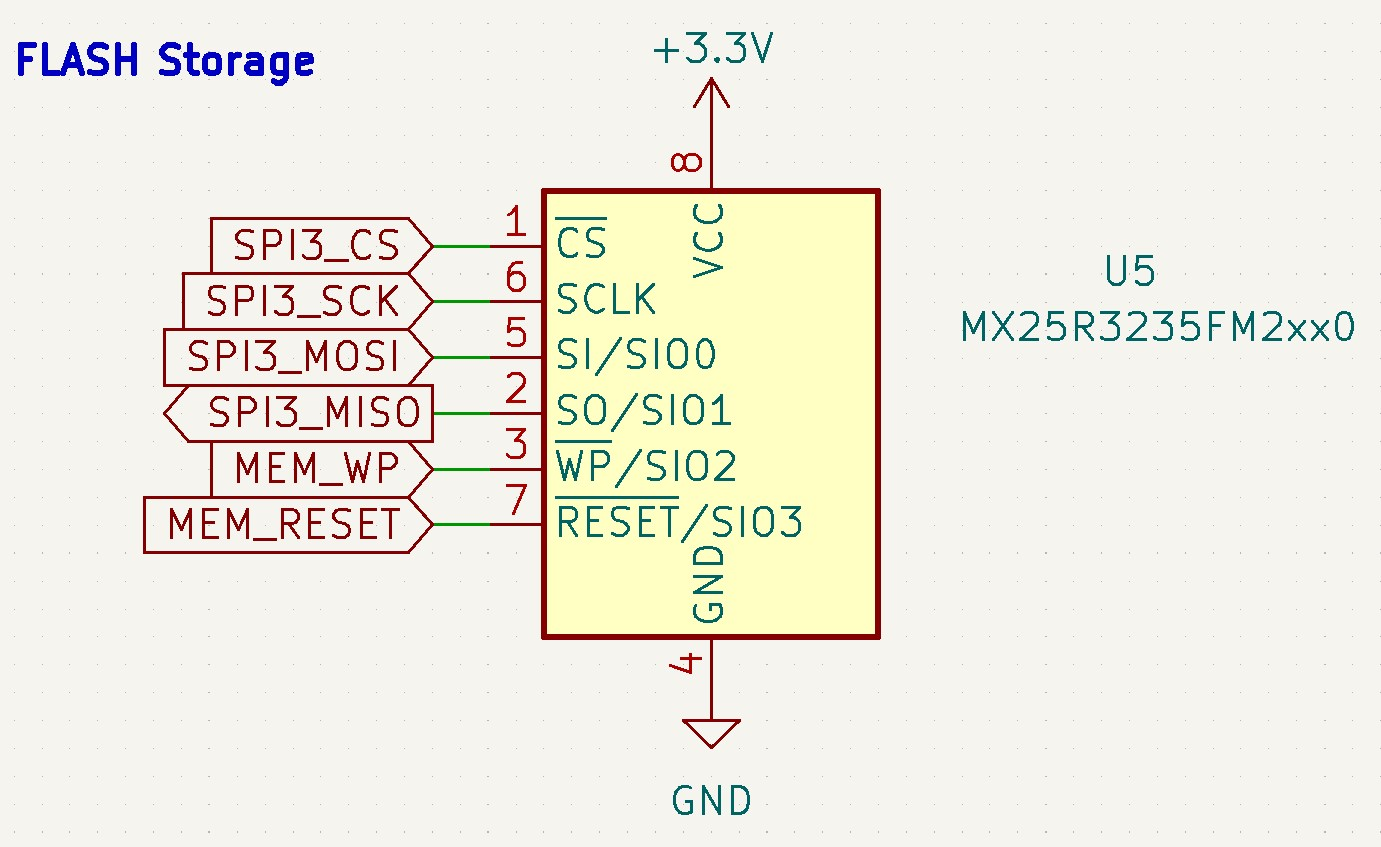
\includegraphics[width=0.8\textwidth]{pictures/flash_memory.jpg}
\end{figure}
Paměť je rozdělena do 64 kB bloků, které jsou poté rozděleny do bloků po 32 kB a ty do 4 kB sektorů. Do paměti je nejmenší možný zápis po 256 B stránkách. Přenosová perioda příchozích 24 bit dat z AD převodníku je $t_s = 208 \ \mu s$ a doba pro zápis celé stránky je $t_{PW} = 850 \ \mu s$. 256 B příchozích z AD převodníku je za $t_p = 256 \times \frac{t_s}{3} \doteq 17.7 \ ms$.
Použitá paměť umožní uložit data s dostatečnou prodlevou před příchozí další 256 B z AD převodníku MCP3561.
\section{Nouzové zastavení}
Přístroj je vybaven obvodem pro připojení nouzového tlačítka.
\begin{figure}[H]
    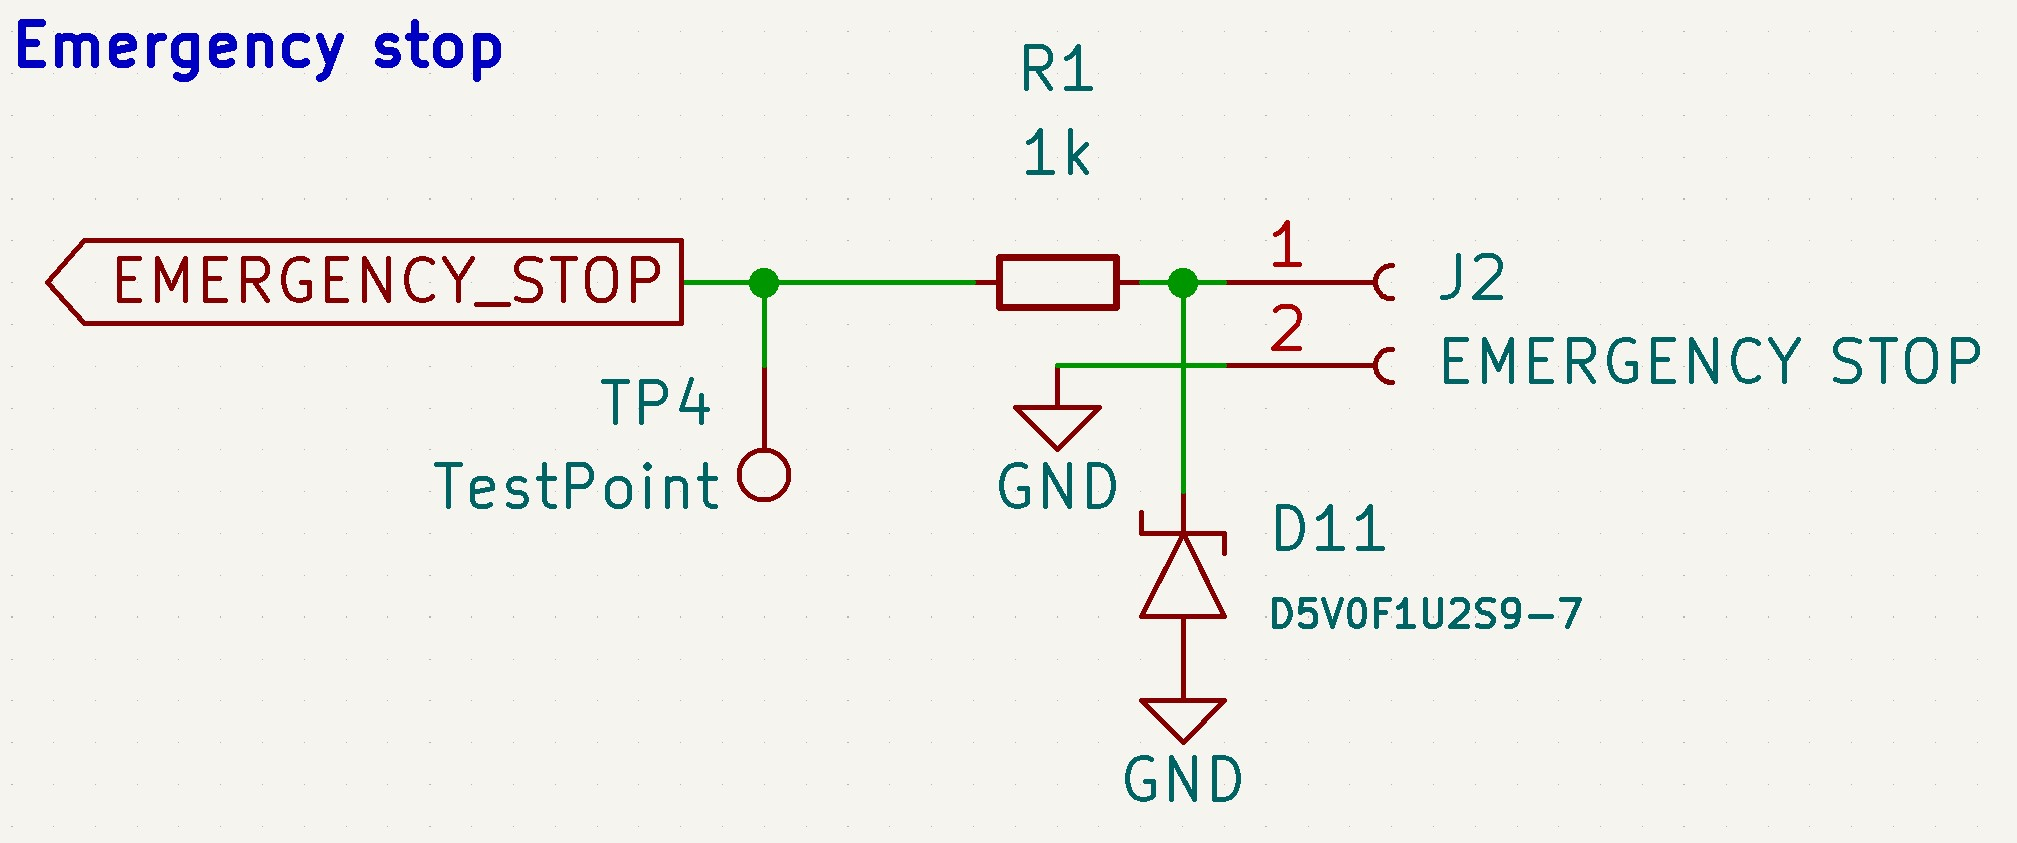
\includegraphics[width=0.9\linewidth]{pictures/e_stop.jpg}
    \caption{Schéma zapojení nouzového tlačítka}
    \label{fig:e_stop}
\end{figure}
Nouzové tlačítko je připojeno ke vstupnímu pinu MCU, které má k dispozici externí přerušení. Pin MCU musí mít pull up rezistor a přerušení nastavené na detekci spádové hrany. Toto nastavení zajistí
detekci odpojeného nouzového tlačítka, přístroj se programově nastaví do stavu nouze a tím uživateli přístroje zabrání spuštění měření bez zabezpečení proti selhání.
\section{Napájení}
Vstupní napětí je $U_{in} = 5 \ V DC$ a poskytuje napájení celého systému. Vstupní napětí je poté pomocí regulátoru napětí s nízkým úbytkem usměrněno na $3.3 \ V$ pro napájení MCU, sensorů a ostatních komponentů.

\begin{figure}[H]
    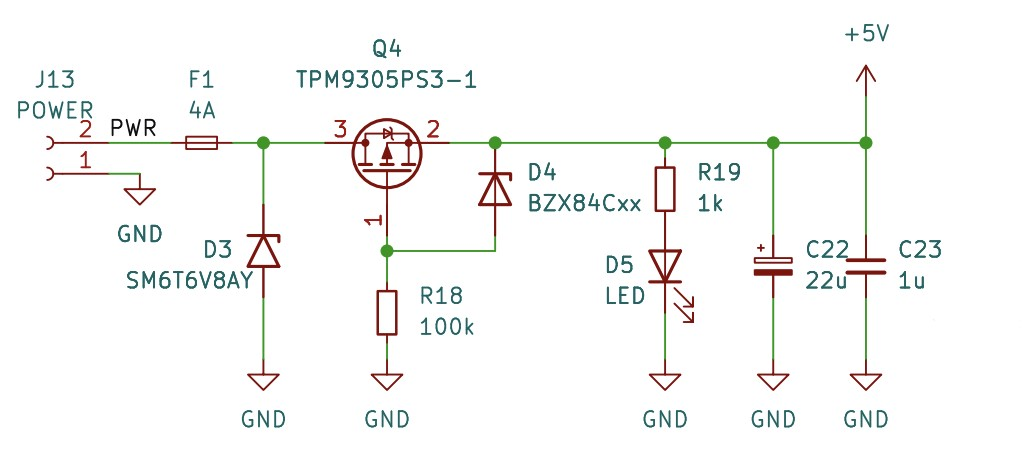
\includegraphics[width=0.9\linewidth]{pictures/power.jpg}
    \caption{Schéma zapojení vstupního napájení}
    \label{fig:power_input}
\end{figure}

Celkový proudový odběr přístroje je popsán v níže uvedené tabulce
\begin{table}[H]
    \label{tab:sum_of_current}
    \caption{Celkový proudový odběr přístroje}
    % \hspace*{-1.2cm}
    \centering
    \begin{ctucolortab}
        \begin{tabular}{cccccc}
            \toprule
            Komponenta              & Název                 & Symbol & Hodnota & Jednotka \\ \midrule
            Diferenční sensor tlaku & Amphenol ELVH-L02D    &        & 35      &          \\
            Sensory tlaku           & NXP MP3V5050GC6U      &        & 20      &          \\
            Uzavírací ventily       & Conjoin CJAV08-2B05A1 &        & 401     &          \\
            Regulační ventily       & JQF4-6A/DC6V          & I      & 214     & mA       \\
            Modul měření BP         & PAR NIBP 2020 UP      &        & 1000    &          \\
            MCU                     & ST M STM32F407ZG6     &        & 109     &          \\
            AD převodník            & Microchip MCP3561     &        & 2.2     &          \\
            FLASH Paměť             & Macronix MX25R3235F   &        & 2       &          \\
            \bottomrule
            $\Sigma$                &                       &        & 1.79    & A        \\
            \bottomrule
        \end{tabular}
    \end{ctucolortab}
\end{table}

Přístroj je opatřen $4 \ A$ pojistkou a ochranou proti opačné polaritě.
Ochrana proti opačné polaritě zajistí při špatném zapojení, aby proud neprotékal přístrojem, ale musí se zajistit, aby ztrátový výkon
\begin{align*}
    W = I^2 R
\end{align*}

byl co nejmenší při správném zapojení. Proto je použit PMOS tranzistor jako ochrana obvodu. Pokud je zdroj zapojen správně, gate je připojen k zemi a source je připojen na kladný terminál, proud bude protékat přes drain. Protože $ U_G = 0 \ V$ a $U_S = U_{in}$, tak
\begin{align*}
    U_{GS} = U_G - U_S
\end{align*}
$U_{GS} = -U_{in} $, proto je potřeba, aby prahové napětí tranzistoru bylo více něž
\begin{align*}
    U_{GS(ON)} > -U_{in}
\end{align*}
Při opačném zapojení napájení $U_S = -U_{in}$ a $ U_G = 0 \ V$, tak  $U_{GS} = U_{in}$ tranzistor je vypnut a přes obvod neprotéká proud.
V návrhu je použit tranzistor TPM9305PS3, který má  $U_{GS(ON)} = -2.5 \ V $,  $I_{D MAX} = -4.1 \ A$ a $R_{DS(ON)} = 52 \ m \Omega$ při $U_{GS} = -4.5 \ V$.
Ztrátový výkon bude při proudovém doběru $I = 2 \ A$
\begin{align*}
    W_{loss} = I^2 R \approx (2)^2 (0.052) =  0.208 \ W
\end{align*}

Mezi $U_G$ a $U_S$ je připojena Zenerova dioda, která zamezí maximální napětí, pro ochranu tranzistoru. Pokud napájecí zdroj bude mít větší napětí něž maximální povolené napětí na $U_{GS}$, zenerova dioda upne $U_{GS}$ na její maximální napětí.
\par
Pro maximální zamezení rušivých jevů a zlepšení EMC jsou připojeny paralelně dva blokovací kondenzátory.
\subsection*{Regulátor napětí}
\begin{figure}[H]
    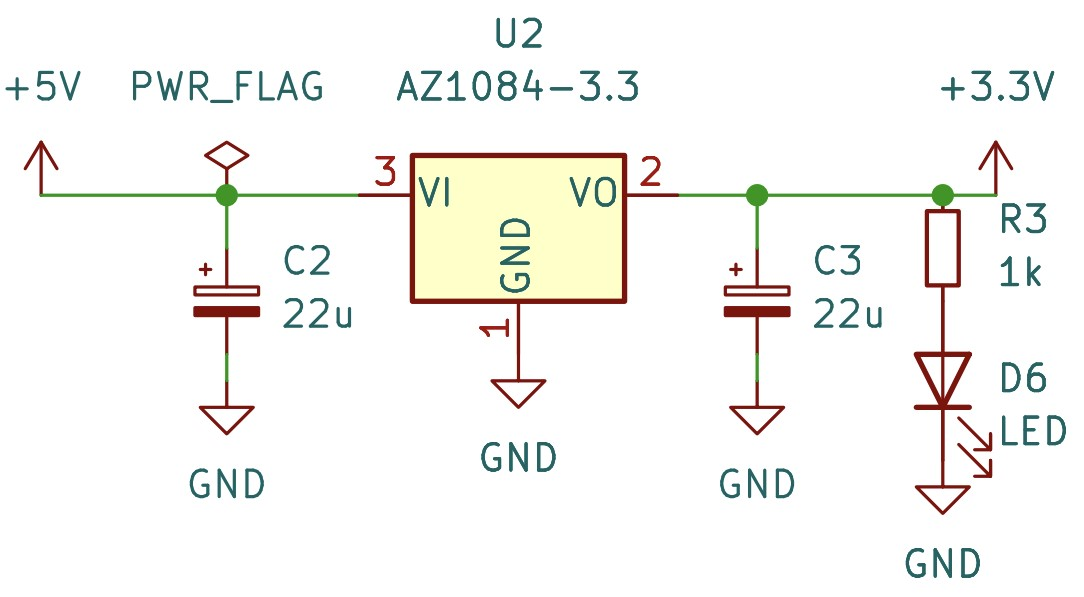
\includegraphics[width=0.9\linewidth]{pictures/ldo_3v3.jpg}
    \caption{Schéma zapojení regulátoru napětí AZ1084-3.3 z 5V na 3.3V}
    \label{fig:stepdown}
\end{figure}
Je použit lineární regulátor napětí s nízkým úbytkem AZ1084-3.3 od firmy Diodes Incorporated.
Vstupní napětí regulátoru je v rozmezí $1.5 \ V \leq U_{in} \leq 12 \ V $, výstupní napětí je fixní na $U_{out} = 3.3 \ V$ a maximální výstupní proud je $I_{out(MAX)} = 5 \ A$. Zapojení regulátoru je podle doporučeného zapojení v katalogovém listu.


